%% LaTeX Template for ISIT 2020
%%
%% by Stefan M. Moser, October 2017
%% 
%% derived from bare_conf.tex, V1.4a, 2014/09/17, by Michael Shell
%% for use with IEEEtran.cls version 1.8b or later
%%
%% Support sites for IEEEtran.cls:
%%
%% http://www.michaelshell.org/tex/ieeetran/
%% http://moser-isi.ethz.ch/manuals.html#eqlatex
%% http://www.ctan.org/tex-archive/macros/latex/contrib/IEEEtran/
%%

\documentclass[conference,letterpaper]{IEEEtran}

%% depending on your installation, you may wish to adjust the top margin:
\addtolength{\topmargin}{9mm}

%%%%%%
%% Packages:
%% Some useful packages (and compatibility issues with the IEEE format)
%% are pointed out at the very end of this template source file (they are 
%% taken verbatim out of bare_conf.tex by Michael Shell).
%
% *** Do not adjust lengths that control margins, column widths, etc. ***
% *** Do not use packages that alter fonts (such as pslatex).         ***
%

\usepackage[utf8]{inputenc} 
\usepackage[T1]{fontenc}
\usepackage{url}
\usepackage{ifthen}
\usepackage{cite}
\usepackage[cmex10]{amsmath} % Use the [cmex10] option to ensure complicance
                             % with IEEE Xplore (see bare_conf.tex)

%% Please note that the amsthm package must not be loaded with
%% IEEEtran.cls because IEEEtran provides its own versions of
%% theorems. Also note that IEEEXplore does not accepts submissions
%% with hyperlinks, i.e., hyperref cannot be used.

\interdisplaylinepenalty=2500 % As explained in bare_conf.tex

\usepackage{bm,amsmath,amssymb,multicol,algorithmic,algorithm,enumitem}
\usepackage{times}
\usepackage{dsfont}
\usepackage{xargs}
\newcounter{protocol}
\makeatletter
\newenvironment{protocol}[1][htb]{%
  \let\c@algorithm\c@protocol
  \renewcommand{\ALG@name}{Protocol}% Update algorithm name
  \begin{algorithm}[#1]%
  }{\end{algorithm}
}
\makeatother
\usepackage{mathtools}  
\usepackage{amsmath}
\usepackage{amssymb}
\usepackage{tabulary}
\usepackage{booktabs}
\usepackage{stmaryrd}
\usepackage{color,wrapfig}
\newtheorem{Fact}{Fact}
\newtheorem{Lemma}{Lemma}
\newtheorem{Prop}{Proposition}
\newtheorem{Theorem}{Theorem}
\newtheorem{Def}{Definition}
\newtheorem{Corollary}{Corollary}
\newtheorem{Conjecture}{Conjecture}
\newtheorem{Property}{Property}
\newtheorem{Observation}{Observation}
%\theorembodyfont{\rmfamily}
\newtheorem{Exa}{Example}
\newtheorem{assumption}{A\!\!}
\newtheorem{assumptionA}{G\!\!}
\newtheorem{Remark}{Remark}


\usepackage{shortcuts_OPT}

%%%%%%
% correct bad hyphenation here
\hyphenation{op-tical net-works semi-conduc-tor}

% ------------------------------------------------------------
\begin{document}
\title{Two-Timescale Stochastic EM Algorithms} 

% %%% Single author, or several authors with same affiliation:
% \author{%
%   \IEEEauthorblockN{Stefan M.~Moser}
%   \IEEEauthorblockA{ETH Zürich\\
%                     ISI (D-ITET)\\
%                     CH-8092 Zürich, Switzerland\\
%                     Email: moser@isi.ee.ethz.ch}
% }


%%% Several authors with up to three affiliations:
\author{%
  \IEEEauthorblockN{Belhal Karimi and Ping Li}
  \IEEEauthorblockA{Cognitive Computing Lab\\
  			Baidu Research \\
			10900 NE 8th St. Bellevue, WA 98004, USA\\
Email: \{belhal.karimi, pingli98\}@gmail.com}
}


\maketitle

%%%%%%
%% Abstract: 
%% If your paper is eligible for the student paper award, please add
%% the comment "THIS PAPER IS ELIGIBLE FOR THE STUDENT PAPER
%% AWARD." as a first line in the abstract. 
%% For the final version of the accepted paper, please do not forget
%% to remove this comment!
%%
\begin{abstract}
The Expectation-Maximization (EM) algorithm is a popular choice for learning latent variable models. 
Variants of the EM have been initially introduced by~\cite{neal1998view}, using incremental updates to scale to large datasets, and by~\cite{wei1990monte, delyon1999}, using Monte Carlo (MC) approximations to bypass the intractable conditional expectation of the latent data for most nonconvex models.
In this paper, we propose a general class of methods called Two-Timescale EM Methods based on a two-stage approach of stochastic updates to tackle an essential nonconvex optimization task for latent variable models.
We motivate the choice of a double dynamic by invoking the variance reduction virtue of each stage of the method on both sources of noise: the index sampling for the incremental update and the MC approximation.
We establish finite-time and global convergence bounds for nonconvex objective functions.
Numerical applications on various models such as a deformable template for \emph{image analysis} or \emph{Gaussian Mixture Models} are also presented to illustrate~our~findings.
\end{abstract}



% \textit{A full version of this paper is available at:}
% \textcolor{magenta}{\url{https://hal.archives-ouvertes.fr/hal-02994707/document} }

\section{Introduction}


Learning latent variable models is critical for modern machine learning problems, see (e.g.,)~\cite{mclachlan2007algorithm} for references.
We formulate the training of such model as the following \emph{empirical risk minimization} problem:
\begin{align} \label{eq:em_motivate}
\begin{split} 
& \min_{ \param \in \Param }~ \overline{\calL} ( \param ) \eqdef  \calL ( \param ) + \Pen (\param)\\
& \text{with}~~\calL ( \param ) = \frac{1}{n} \sum_{i=1}^n \calL_i( \param) \eqdef  \frac{1}{n} \sum_{i=1}^n \big\{ - \log g( y_i ; \param ) \big\}\eqs,
\end{split} 
\end{align}
where $\{y_i\}_{i=1}^n$ are observations, $\Param \subset \rset^d$ is the parameters set and $\Pen : \Param \rightarrow \rset$ is a smooth regularizer.
The objective $ \overline{\calL} ( \param )$ is possibly \emph{nonconvex} and is assumed to be lower bounded. 
In the latent data model, the likelihood $g(y_i ; \param)$, is the marginal of the complete~data likelihood defined as $f(z_i,y_i; \param)$, $g(y_i; \param) = \int_{\Zset} f (z_i,y_i;\param) \mu(\rmd z_i)$, where $\{ z_i \}_{i=1}^n$ are the latent variables.
In this paper, we assume that the complete model belongs to the curved exponential family~\cite{efron1975defining}, \textit{i.e.}:
\beq \label{eq:exp}
f(z_i,y_i; \param) = h  (z_i,y_i) \exp \big( \pscal{S(z_i,y_i)}{\phi(\param)} - \psi(\param) \big)\eqs,
\eeq
where $\psi(\param)$, $h(z_i,y_i)$ are scalar functions, $\phi(\param) \in \rset^k$ is a vector function, and $\{S(z_i,y_i) \in \rset^k\}_{i=1}^n$ is the vector of sufficient statistics.
Batch EM~\cite{dempster1977Maximum, wu1983convergence}, the method of reference for \eqref{eq:em_motivate}, is comprised of two steps. 
The \textsf{E-step} computes the conditional expectation of the statistics of~\eqref{eq:exp}, noted $\overline{\bss}(\param)= \frac{1}{n} \sum_{i=1}^n \overline{\bss}_i(\param)$ where for $i \in \inter$:
\begin{align}\label{eq:definition-overline-bss}
 \overline{\bss}_i(\param)= \int_{\Zset} S(z_i,y_i) p(z_i|y_i;\param) \mu(\rmd z_i) \eqsp,
\end{align}
%\begin{align}\label{eq:definition-overline-bss}
%\begin{split} 
%& \overline{\bss}(\param)= \frac{1}{n} \sum_{i=1}^n \overline{\bss}_i(\param) \\
%& \text{where}  \quad \overline{\bss}_i(\param)= \int_{\Zset} S(z_i,y_i) p(z_i|y_i;\param) \mu(\rmd z_i) \eqsp,
%\end{split} 
%\end{align}
and the \textsf{M-step} is given by
\begin{align}\label{eq:mstep}
\overline{\param}( \overline{\bss}(\param) ) \eqdef \argmin_{ \vartheta \in \Param } ~\big\{ \Pen( \vartheta ) + \psi( \vartheta) - \pscal{ \overline{\bss}(\param)}{ \phi ( \vartheta) } \big\} \eqsp.
\end{align}


Two caveats of this method are the following: {\sf(a)} with the explosion of data, the first step of the EM is computationally inefficient as it requires, at each iteration, a full pass over the dataset; and {\sf(b)} the complexity of modern models makes the expectation in \eqref{eq:definition-overline-bss} intractable. 
To the best of our knowledge, both challenges have been addressed separately.

\vspace{0.08in}
\noindent \textbf{Prior Work:} Inspired by stochastic optimization procedures,~\cite{neal1998view,cappe2009line} develop respectively an incremental and an online variant of the \textsf{E-step} in models where the expectation is computable, and were then extensively used and studied in~\cite{nguyen2020mini, liang2009online,cappe2011online}.
Some improvements of those methods have been provided and analyzed, globally and in finite-time, in~\cite{karimi2019global} where variance reduction techniques taken from the optimization literature have been efficiently applied to scale the EM algorithm to large datasets.
Regarding the computation of the expectation under the posterior distribution, the Monte Carlo EM (MCEM) has been introduced in~\cite{wei1990monte} where a Monte Carlo (MC) approximation for this expectation is computed. A variant of that algorithm is the Stochastic Approximation of the EM (SAEM) in~\cite{delyon1999} leveraging the power of Robbins-Monro update~\cite{robbins1951stochastic} to ensure pointwise convergence of the vector of estimated parameters using a decreasing stepsize rather than increasing the number of Monte Carlo samples.
The MCEM and the SAEM have been successfully applied in mixed effects models~\cite{mcculloch1997maximum,hughes1999mixed,baey2016nonlinear} or to do inference for joint modeling of time to event data coming from clinical trials in~\cite{das2010Inferences}, unsupervised clustering in~\cite{ngChoice2003}, variational inference of graphical models in~\cite{BleiVariational2017} among other applications.
An incremental variant of the SAEM was proposed in~\cite{kuhn2019properties} showing positive empirical results but its analysis is limited to asymptotic consideration. 


\vspace{0.08in}
\noindent \textbf{Contributions:} This paper \textit{introduces} and \textit{analyzes} a new class of methods which purpose is to update two proxies for the target expected quantities in a two-timescale manner. 
Those approximated quantities are then used to optimize the objective function \eqref{eq:em_motivate} for modern examples and settings using the \textsf{M-step} of the EM algorithm.
Our main contributions are:
\begin{itemize}
\item We propose a two-timescale method based on \textsf{(i)} Stochastic Approximation (SA), to alleviate the problem of computing MC approximations, and on \textsf{(ii)} Incremental updates, to scale to large datasets. We describe in details the edges of each level of our method based on variance reduction arguments. Such class of algorithms has two advantages. First, it naturally leverages variance reduction and Robbins-Monro type of updates to tackle large-scale and highly nonlinear learning tasks. Then, it gives a simple formulation as a \textit{scaled-gradient method} which makes the analysis and implementation accessible.
\item We also establish global, \ie independent of the initialization, and finite-time (true at each iteration) upper bounds on a classical sub-optimality condition in the nonconvex literature~\cite{jain2017non, ghadimi2013stochastic}, \ie\ the second order moment of the gradient of the objective function. 
We discuss the double dynamic of those bounds due to the two-timescale property of our algorithm update and we theoretically show the advantages of introducing variance reduction in our \emph{Stochastic Approximation}~\cite{robbins1951stochastic} scheme.
\item We stress on the originality of our theoretical findings including such MC sampling noise contrary to existing studies related to the EM where the expectations are computed exactly. 
Adding a layer of MC approximation and the stochastic approximation step to reduce its variance introduce some new technicalities and challenges that need careful considerations and constitues the originality of our paper on the algorithmic and theoretical plans.
\end{itemize}


\section{Two-Timescale Stochastic EM Algorithms}\label{sec:tts}


We recall and formalize in this section the different methods found in the literature that aim at solving the intractable expectation and the large-scale problem. 
We then introduce our method that efficiently tackles the optimization \eqref{eq:em_motivate}.


\subsection{Monte Carlo Integration and Stochastic Approximation} 


As mentioned in the Introduction, for complex and possibly nonconvex models, the expectation under the posterior distribution defined in \eqref{eq:definition-overline-bss} is not tractable. 
In that case, the first solution involves computing a Monte Carlo integration of that expectation. 
For all $ i \in \inter$, where $\inter \eqdef \{1, \cdots, n\}$, draw $\{z_{i,m} \sim p(z_i|y_i;\theta)\}_{m=1}^{M}$ samples and compute the MC integration of $\tilde{S}$ of $\overline{\bss}(\param)$ defined by \eqref{eq:definition-overline-bss}:
\beq\label{eq:mcstep}
\textsf{MC-step}:~ \tilde{S} \eqdef \frac{1}{n} \sum_{i=1}^n\frac{1}{M} \sum_{m=1}^M S(z_{i,m}, y_i)\eqs.
\eeq
Then update the parameter via the maximization function $\overline{\param}(\tilde{S} )$.
This algorithm bypasses the intractable expectation issue but is rather computationally expensive since in order to reach point wise convergence, $M$ needs to be increasingly large.
An alternative to that stochastic algorithm is to use a Robbins-Monro (RM) type of update.
We denote, at iteration $k$, the number of samples $M_k$ and the following MC approximation by $\tilde{S}^{(k+1)}$:
\beq\label{eq:stats}
\begin{split}
 \tilde{S}^{(k+1)} \eqdef \frac{1}{n} \sum_{i=1}^n \tilde{S}^{(k+1)}_i = \frac{1}{n} \sum_{i=1}^n\frac{1}{M_k} \sum_{m=1}^{M_k} S(z_{i,m}^{(k)}, y_i) \eqs,
\end{split}
\eeq
where $z_{i,m}^{(k)} \sim p(z_i|y_i;\theta^{(k)})$.
Then, the RM update of the sufficient statistics $\hat{\bss}^{(k+1)}$ reads:
\beq\label{eq:rmstep}
\textsf{SA-step}:~ \hat{\bss}^{(k+1)} =  \hat{\bss}^{(k)}  + \gamma_{k+1}(\tilde{S}^{(k+1)} - \hat{\bss}^{(k)} )\eqs,
\eeq
where $\{ \gamma_{k} \}_{k>1} \in (0,1)$ is a sequence of decreasing stepsizes to ensure asymptotic convergence.
The combination of \eqref{eq:stats}, \eqref{eq:rmstep} and \eqref{eq:mstep} is called the Stochastic Approximation of the EM (SAEM) and has been shown to converge to a maximum likelihood of the observations under very general conditions~\cite{delyon1999}.
In simple scenarios, the samples $\{z_{i,m}\}_{m=1}^{M}$ are conditionally independent and identically distributed with distribution $p(z_i,\theta)$.
Nevertheless, in most cases, since the loss function between the observed data $y_i$ and the latent variable $z_i$ can be nonconvex, sampling exactly from this distribution is not an option and the MC batch is sampled by Markov Chain Monte Carlo (MCMC) algorithm~\cite{meyn2012markov, brooks2011handbook}.
It has been proved in~\cite{kuhn2004coupling} that \eqref{eq:rmstep} converges almost surely when coupled with an MCMC procedure. 
%\noindent \textbf{Role of the stepsize $\gamma_k$:}  The sequence of decreasing positive integers $\{ \gamma_{k} \}_{k>1}$ controls the convergence of the algorithm.
%It is inefficient to start with small values for the stepsize $\gamma_k$ and large values for the number of simulations $M_k$. 
%Rather, it is recommended that one decreases $\gamma_k$, as in $\gamma_k = 1/k^\alpha$, with $\alpha \in (0,1)$, and keeps a constant and small number $M_k$ bypassing the computationally involved sampling step in \eqref{eq:mcstep}.
% In practice, $\gamma_k$ is set equal to $1$ during the first few iterations to let the iterates explore the parameter space without memory and converge quickly to a neighborhood of the target estimate. 
% The Stochastic Approximation is performed during the remaining iterations ensuring the almost sure convergence of the vector of estimates.
This RM type of update constitutes the \textit{first level} of our algorithm, needed to temper the variance and noise introduced by the Monte Carlo integration.
In the next section, we derive variants of this algorithm to adapt to the sheer size of data of today's applications and formalize the \textit{second level} of our class of two-timescale EM methods.


\subsection{Incremental and Two-Stage Stochastic EM Methods} \label{sec:sEM}

Efficient strategies to scale to large datasets include incremental~\cite{neal1998view} and variance reduced~\cite{chen2018stochastic, johnson:zhang:2013} methods.
We explicit a general update that covers those latter variants and that represents the \textit{second level} of our algorithm, \ie the incremental update of the noisy statistics $\tilde{S}^{(k+1)}$ in \eqref{eq:stats}. 
Instead of computing its full batch $\tilde{S}^{(k+1)}$ as in \eqref{eq:stats}, the MC approximation is incrementally evaluated through $\stt^{(k+1)}$ as:
\beq \label{eq:sestep}
\textsf{Inc-step}:~\stt^{(k+1)} = \stt^{(k)} + \rho_{k+1} \big( \StocEstep^{(k+1)}- \stt^{(k)}  \big)\eqs.
\eeq
Note that $\{ \rho_{k} \}_{k>1} \in (0,1)$ is a sequence of stepsizes, $\StocEstep^{(k)}$ is a proxy for $\tilde{S}^{(k)}$ defined in \eqref{eq:stats}.
If the stepsize is equal to $1$ and $\StocEstep^{(k)} = \tilde{S}^{(k)}$, i.e., computed in a full batch manner as in \eqref{eq:stats}, then we recover the SAEM algorithm.
Also if $\rho_{k}=1$, $\gamma_{k}=1$ and $\StocEstep^{(k)} = \tilde{S}^{(k)}$, then we recover the MCEM.

 \begin{protocol}[H]
  \floatname{algorithm}{Table}
\caption{Proxies for the Incremental-step~\eqref{eq:sestep}}\label{alg:prox}
  \begin{algorithmic}[1]
  \STATE \textsf{\ISAEM\ }$\hspace{0.7cm} \StocEstep^{(k+1)} = \StocEstep^{(k)} + n^{-1} \big( \tilde{S}_{i_k}^{(k)}  - \tilde{S}_{i_k}^{(\tau_{i_k}^k)} \big) \label{eq:isaem}$
    \STATE \textsf{\SAEMVR\ }$\hspace{0.5cm} \StocEstep^{(k+1)}  = \stt^{(\ell(k))} +  \big( \tilde{S}_{i_k}^{(k)}  -\tilde{S}_{i_k}^{(\ell(k))}   \big) \label{eq:vrsaem}$
      \STATE \textsf{\FISAEM\ }$\hspace{0.6cm} \StocEstep^{(k+1)} = \overline{\StocEstep}^{(k)} + \big( \tilde{S}_{i_k}^{(k)}  - \tilde{S}_{i_k}^{(t_{i_k}^k)} \big) \label{eq:fisaem}$\\
             $ \hspace{1.95cm} \overline{\StocEstep}^{(k+1)} = \overline{\StocEstep}^{(k)} + n^{-1} \big( \tilde{S}_{j_k}^{(k)}  - \tilde{S}_{j_k}^{(t_{j_k}^k)} \big)$
  \end{algorithmic}
\end{protocol}
\vspace{0.08in}
\noindent \textbf{Remarks on Table~\ref{alg:prox}:} For all methods, we define a random index noted $i_k \in \inter$ and drawn at iteration $k$, and $\tau_i^k = \max \{ k' : i_{k'} = i,~k' < k \}$ as the iteration index where $i \in \inter$ is last drawn prior to iteration $k$.



Note that the proposed \FISAEM\ method draws \emph{two} indices \emph{independently} and uniformly as $i_k, j_k \in \inter$. 
Thus, we define $t_j^k = \{ k' : j_{k'} = j , k' < k \}$ to be the iteration index where the sample $j \in \inter$ is last drawn as $j_k$ prior to iteration $k$ in addition to $\tau_i^k$ which was defined \wrt $i_k$.


Recall that $\tilde{S}_{i_k}^{(k)} \eqdef  \frac{1}{M_k} \sum_{m=1}^{M_k} S(z_{i_k,m}^{(k)}, y_{i_k})$ where $z_{i_k,m}^{(k)}$ are samples drawn from $ p(z_{i_k}|y_{i_k};\theta^{(k)})$.
The stepsize in~\eqref{eq:sestep} is set to $\rho_{k+1} = 1$ for the \ISAEM\ method where we initialize with $\StocEstep^{(0)} = \tilde{S}^{(0)}$; $\rho_{k+1} = \rho$ is  constant for the \SAEMVR\ and \FISAEM\ methods. Note that we initialize as follows $\overline{\StocEstep}^{(0)} = \tilde{S}^{(0)}$ for the \FISAEM\ which can be seen as a slightly modified version of SAGA inspired by~\cite{reddi2016fast}.
For \SAEMVR\, we set an epoch size of $m$ and we define $\ell(k) \eqdef m \lfloor k/m \rfloor$ as the first iteration number in the epoch that iteration $k$ is in.


\vspace{0.08in}
\noindent \textbf{Two-Timescale Stochastic EM methods:}
We now introduce the general method derived using the two variance reduction techniques described above.
Algorithm~\ref{alg:ttsem} leverages both levels \eqref{eq:rmstep} and \eqref{eq:sestep} in order to output a vector of fitted parameters $\hat{\param}^{({\sf K}_{\sf f })}$ where ${\sf K}_{\sf f }$ denotes the total number of iterations.
\begin{algorithm}[H]
\caption{Two-Timescale Stochastic EM methods.}\label{alg:ttsem}
  \begin{algorithmic}[1]
  \STATE \textbf{Input:} $\hat{\param}^{(0)} \leftarrow 0$, $\hat{\bss}^{(0)} \leftarrow \tilde{S}^{(0)}$, $\{\gamma_k\}_{k>0}$, $\{\rho_k\}_{k>0}$ and $ {\sf K}_{\sf f }\in \mathbb{N}^*$.
%  \STATE Set the terminating iteration number, $K \in \{0,\dots,{\sf K}_{\sf f }-1\}$, as a discrete r.v.~with:\vspace{-.1cm}
%  \beq \label{eq:random}
%   P( K = k ) = \frac{ \gamma_{k} }{\sum_{\ell=0}^{{\sf K}_{\sf f }-1} \gamma_\ell} = \frac{\gamma_k}{{\sf P}_{\sf m}}\eqs.\vspace{-.2cm} 
%  \eeq
  \FOR {$k=0,1,2,\dots, {\sf K}_{\sf f } - 1$}
  \STATE Draw index $i_k \in \inter$ uniformly (and $j_k \in \inter$ for \FISAEM).
     \STATE Compute $\tilde{S}_{i_k}^{(k)}$ using the {\sf MC-step} \eqref{eq:mcstep},  for the drawn indices.
   \STATE Compute the surrogate sufficient statistics $\StocEstep^{(k+1)}$ using Lines~\ref{eq:isaem}, \ref{eq:vrsaem} or \ref{eq:fisaem} in Table~\ref{alg:prox}.
   \STATE Compute $\stt^{(k+1)}$ and $\hat{\bss}^{(k+1)}$ using resp. \eqref{eq:sestep} and \eqref{eq:rmstep}:
\beq \label{eq:twolevels}
\begin{split}
& \stt^{(k+1)} = \stt^{(k)} + \rho_{k+1} \big( \StocEstep^{(k+1)}- \stt^{(k)}  \big)\\
&  \hat{\bss}^{(k+1)} =  \hat{\bss}^{(k)}  + \gamma_{k+1}(\stt^{(k+1)} - \hat{\bss}^{(k)} )
\end{split}
\eeq
   \STATE Update $\hat{\param}^{(k+1)} = \overline{\param}(  \hat{\bss}^{(k+1)}) $ via the {\sf M-step} \eqref{eq:mstep}.
\ENDFOR
  \end{algorithmic}
\end{algorithm}
The update in \eqref{eq:twolevels} is said to have a \emph{two-timescale} property as the stepsizes satisfy $\lim_{k \to \infty} \gamma_k/\rho_k < 1$ such that $ \tilde{S}^{(k+1)} $  is updated at a faster time-scale, determined by $\rho_{k+1}$, than $\hat{\bss}^{(k+1)}$, determined by $\gamma_{k+1}$.
The next section introduces the main results of this paper and establishes global and finite-time bounds for the three different updates of our scheme. 
We recall the main notations introduced previously:\vspace{-0.05in}

\begin{table}[htbp]
%\caption{Table of Notations}
\begin{center}% used the environment to augment the vertical space
% between the caption and the table
\begin{tabular}{r c p{7cm} }
\toprule
$\tilde{S}$ & $\triangleq$ &  MC approximation of $\overline{\bss}$, defined in \eqref{eq:definition-overline-bss}, at $i \in \inter$\\
$\StocEstep$ & $\triangleq$ & proxy of the MC approximation $\tilde{S}$ computed via Table~\ref{alg:prox}\\  
$\stt$ & $\triangleq$ & variance-reduced quantity in~\eqref{eq:sestep} and related to stepsize $\rho$\\
$\hat{\bss}$ & $\triangleq$ & statistics resulting from the procedure in~\eqref{eq:rmstep} and related to $\gamma$\\
\bottomrule
\end{tabular}
\end{center}
\label{tab:notations}
\end{table}

\vspace{-0.05in}

\section{Finite Time Analysis of Two-Timescale EMs} \label{sec:mainanalysis}
Following~\cite{cappe2009line}, it can be shown that stationary points of the objective function \eqref{eq:em_motivate} corresponds to the stationary points of the following \textit{nonconvex} Lyapunov function:
\beq\label{eq:em_sspace}
\min_{ {\bss} \in \Sset }~  V ( {\bss} ) \eqdef \overline\calL( \op(\bss) ) =  \frac{1}{n} \sum_{i=1}^n {\cal L}_i (  \op(\bss) )+ \Pen (  \op(\bss) ) \eqs,
\eeq
that we propose to study in this article.


\subsection{Assumptions and Intermediate Lemmas}


Several important assumptions required to derive convergence guarantees are given in the following:
\begin{assumption}\label{ass:compact}
The sets $\Zset, \Sset$ are compact. There exist $C_{\Sset}, C_{\Zset}$ such that:
\beq \textstyle \notag
\begin{split}
& C_{\Sset} \eqdef \max_{ \bss, \bss' \in \Sset } \| \bss - \bss' \| < \infty,\\
& C_{\Zset} \eqdef \max_{i \in \inter} \int_{\Zset} | S(z,y_i) | \mu( \rmd z ) < \infty.
\end{split}
\eeq
\end{assumption}

\begin{assumption}\label{ass:expected}
For any $i \in \inter$, $z \in \Zset$, $\param, \param' \in {\rm int} (\Param)^2$ (the interior of $\Param$), we have $\big| p( z | y_i; \param ) - p( z | y_i; \param' ) \big| \leq  \Lip{p} \| \param - \param' \|$.
\end{assumption}
We also recall that we consider curved exponential family models such that the objective function satisfies:
\begin{assumption} \label{ass:reg}
For any $\bm{s} \in \Sset$, the function $\param \mapsto L(s,\param) \eqdef \Pen( \param ) + \psi( \param) - \pscal{ \bss}{ \phi ( \param) }$ admits a unique global minimum $\mstep{\bss} \in {\rm int}(\Param)$.

In addition, $\jacob{\phi}{\param}{\overline{\param}(\bss )}$, the Jacobian of the function $\phi$ at $\param$, is full rank, $\Lip{p}$-Lipschitz and $\overline{\param}( \bss )$ is $\Lip{t}$-Lipschitz.
\end{assumption}
We denote by $\hess{L}{\param}(\bss,\param)$ the Hessian (w.r.t to $\param$ for a given value of $\bss$) of the function $\param \mapsto L(\bss,\param)= \Pen(\param) + \psi(\param) -\pscal{\bss}{\phi(\param)}$, and define $\operatorname{B}( \bss ) \eqdef\jacob{ \phi }{ \param }{ \mstep{\bss} } \Big( \hess{L}{\param}( {\bss},  \mstep{\bss} )  \Big)^{-1} \jacob{ \phi }{ \param }{ \mstep{\bss} }^\top$.
\begin{assumption}\label{ass:eigen}
It holds that $ \upsilon_{\max} \eqdef \sup_{\bss \in \Sset} \| \operatorname{B}( \bss ) \| < \infty$ and $0 < \upsilon_{\min}  \eqdef \inf_{\bss \in \Sset} \lambda_{\rm min} ( \operatorname{B}( \bss ) )$.
There exists a constant $\Lip{b}$ such that for all $\bss, \bss' \in \Sset^2$, we have $ \| \operatorname{B}( \bss ) - \operatorname{B}( \bss' )  \| \leq \Lip{b} \| {\bss} - {\bss}' \|$.
\end{assumption}
The class of algorithms we develop in this paper is composed of two levels where the second stage corresponds to the variance reduction trick used in~\cite{karimi2019global} in order to accelerate incremental methods and reduce the variance introduced by the index sampling. 
The first stage is the Robbins-Monro update that aims at reducing the Monte Carlo noise of $\tilde{S}^{(k+1)}$ at iteration $k$:
\beq\label{eq:mcerror}
\eta_{i}^{(k)} \eqdef \tilde{S}_{i}^{(k)} -  \overline{\bss}_i(\vartheta^{(k)})\quad  \textrm{for all} \quad  i \in \inter \quad \textrm{and} \quad  k > 0 \eqs.
\eeq
For instance, we consider that the MC approximation is unbiased if for all $ i \in \inter$ and $m \in [M]$, the samples $z_{i,m} \sim p(z_i|y_i;\theta)$ are i.i.d. under the posterior distribution, \ie $\EE[\eta_{i}^{(k)}|{\cal F}_k] = 0$ where  ${\cal F}_k$ is the filtration up to iteration $k$.
The following results are derived under the assumption that the fluctuations implied by the approximation are bounded:
%\begin{assumption}\label{ass:mcerror}
%There exist a positive sequence of MC batch size $\{M_r\}_{r > 0}$ and constants $(c, c_{\eta})$ such that for all $k >0$, $i \in \inter$ and $\vartheta \in \Theta$:
%\beq\label{eq:boundederror}
%\EE [\| \eta_{i}^{(r)}\|^2 ] \leq \frac{c_{\eta}}{M_r} \quad \textrm{and} \quad \EE[\| \EE[\eta_{i}^{(r)}|{\cal F}_r]\|^2] \leq \frac{c}{M_r}\eqs.
%\eeq
%\end{assumption}\vspace{-0.1in}
\begin{assumption}\label{ass:mcerror}
For all $k >0$, $i \in \inter$, it holds: 
$\EE [\| \eta_{i}^{(k)}\|^2 ] < \infty \quad \textrm{and} \quad \EE[\| \EE[\eta_{i}^{(k)}|{\cal F}_k]\|^2] < \infty \eqs.$
\end{assumption}
Note that typically, the controls exhibited above are vanishing when the number of MC samples $M_k$ increases~with~$k$.
%We now state two important results on the Lyapunov function; its smoothness:
%\begin{Lemma} \label{lem:smooth}
%\cite{karimi2019global} Assume A\ref{ass:compact}-A\ref{ass:eigen}.  
%For all $\bss,\bss' \in \Sset$ and $i \in \inter$, we have
%\beq \label{eq:smooth}
%\| \overline{\bss}_i ( \overline{\param} ({\bss})) - \overline{\bss}_i ( \overline{\param} ({\bss}' )) \| \leq \Lip{{\bss}} \| {\bss} - {\bss}' \|,~~\| \grd  V ( {\bss} ) - \grd  V ( {\bss}' ) \| \leq \Lip{V} \| {\bss} - {\bss}' \|\eqs,
%\eeq
%where $\Lip{\bss} \eqdef C_{\Zset} \Lip{p} \Lip{t}$ and $\Lip{V}  \eqdef \upsilon_{\max} \big( 1 + \Lip{{\bss}} \big) + \Lip{b} C_{\Sset}$.
%\end{Lemma}
%We also establish a growth condition on the gradient of $V$ related to the mean field of the algorithm:
%\begin{Lemma}\label{lem:growth}
%Assume A\ref{ass:reg} and A\ref{ass:eigen}. For all $\bss \in \Sset$,
%\beq \label{eq:semigrad}
%\upsilon_{\min}^{-1} \pscal{\grd V ( {\bss} ) }{ {\bss} - \os( \op ({\bss})) } \geq \| {\bss} - \os( \op ({\bss})) \|^2 \geq \upsilon_{\max}^{-2} \| \grd V ( {\bss} ) \|^2\eqs.
%\eeq
%\end{Lemma}

We present in the following sections a finite-time and global (\ie independent of the initialization) analysis of both the incremental and two-timescale variants our method. 


\subsection{Global Convergence of Incremental Stochastic EM}


The following result for the \ISAEM\ algorithm is derived under the control of the Monte Carlo fluctuations as described by Assumption A\ref{ass:mcerror} and is built upon an intermediary Lemma, found in the full version paper, characterizing the quantity of interest $( \stt^{(k+1)} - \hat{\bss}^{(k)} )$:
%\begin{Lemma}\label{lem:meanfield_isaem}
% Assume A\ref{ass:compact}. The \ISAEM\ update~\eqref{eq:isaem} is equivalent to the following update on the statistics $\hat{\bss}^{(k+1)} =  \hat{\bss}^{(k)}  + \gamma_{k+1} \big(  \sum_{i=1}^n \tilde{S}_i^{(\tau_i^k)} - \hat{\bss}^{(k)} \big)$.
%Also:
%\beq\notag
%\EE[\stt^{(k+1)} - \hat{\bss}^{(k)}] = \EE[\overline{\bss}^{(k)} - \hat{\bss}^{(k)}] + \left(1 - \frac{1}{n} \right) \EE\left[\frac{1}{n} \sum_{i=1}^n \tilde{S}_i^{(\tau_i^k)}- \overline{\bss}^{(k)}\right]  +\frac{1}{n}\EE[\eta_{i_k}^{(k+1)}]\eqsp,
%\eeq
%where $\overline{\bss}^{(k)}$ is defined by \eqref{eq:definition-overline-bss} and $\tau_i^k = \max \{ k' : i_{k'} = i,~k' < k \}$.
%\end{Lemma}
%Then, the following non-asymptotic convergence rate can be derived for the \ISAEM\ algorithm:
\begin{Theorem}\label{thm:isaem}
Assume A\ref{ass:compact}-A\ref{ass:mcerror}.
Consider the \ISAEM\ sequence $\{\hat{\bss}^{(k)}\}_{k>0} \in \mathcal{S}$ obtained with $\rho_{k+1}=1$ for any $k \leq {\sf K}_{\sf f }$ where ${\sf K}_{\sf f } > 0$. 
Let $\{\gamma_{k} = 1/(k^a \alpha c_1 \overline{L})\}_{k>0}$, where $a \in (0,1)$, be a sequence of stepsizes, $c_1 = \upsilon_{\min}^{-1}$, $\alpha = \max\{8, 1+6\upsilon_{\min}\}$, $\overline{L} = \max\{ \Lip{\bss} , \Lip{V} \}$, $\beta = c_1 \overline{L}/n$, then:
\beq\notag
\begin{split}
& \upsilon_{\max}^{-2}\sum_{k=0}^{{\sf K}_{\sf f }} \tilde{\alpha}_k \EE [\|\grd V( \hs{k} )\|^2]\\
&  \leq   \EE  [V( \hs{0} ) - V( \hs{{\sf K}_{\sf f }} ) ] + \sum_{k=0}^{{\sf K}_{\sf f }-1} \tilde{\Gamma}_k         \EE [\| \eta_{i_k}^{(k)}\|^2] \eqs.
\end{split}
\eeq
\end{Theorem} 
Note that, in Theorem~\ref{thm:isaem}, the convergence bound is composed of an initialization term $V( \hs{0} ) - V( \hs{{\sf K}_{\sf f }} )$ and suffers from the Monte Carlo noise introduced by the posterior sampling step, see the second term on the RHS of the inequality. 
We observe, in the next section, that when variance reduction is applied ($\rho_k < 1$), a second phase of convergence manifests.


\subsection{Global Convergence of Two-Timescale Stochastic EM}


We now deal with the analysis of Algorithm~\ref{alg:ttsem} when variance reduction is applied \ie\ $\rho <1$.
Two important intermediate Lemmas are developed in the full version of this paper and lead to the finite-time bounds for the \SAEMVR\ and the \FISAEM\ methods that we describe below.
%We first derive an identity for the drift term of the \SAEMVR\ :
%\begin{Lemma}\label{lem:auxvrsaem}
%Consider the \SAEMVR\ update~\eqref{eq:vrsaem} with $\rho_k = \rho$, it holds for all $k>0$ 
%\beq\notag
%\begin{split}
%  \EE [\| \hs{k} - \stt^{(k+1)}\|^2 ] \leq& 2\rho^2 \EE[ \| \hs{k} - \os^{(k)} \|^2] +  2\rho^2\Lip{\bss}^2 \EE[ \| \hs{k} - \hs{\ell(k)} \|^2 ]\\
%  &+2(1-\rho)^2 \EE[ \| \hs{(k)} - \stt^{(k)} \|^2 ]+ 2\rho^2\EE[\|\eta_{i_k}^{(k+1)} \|^2]\eqs,
%\end{split}
%\eeq
%where we recall that $\ell(k)$ is the first iteration number in the epoch that iteration $k$ is in.
%\end{Lemma}
%The second one derives an identity for the quantity $\EE[ \| \hs{k} - \stt^{(k+1)}   \|^2 ]$ using the \FISAEM\ update:
%\begin{Lemma}\label{lem:aux1}
%Consider the \FISAEM\ update~\eqref{eq:fisaem} with $\rho_k = \rho$. It holds for all $k>0$ that
%\beq\notag
%\begin{split}
%  \EE [\| \hs{k} - \stt^{(k+1)}\|^2 ] \leq& 2\rho^2 \EE[ \| \hs{k} - \os^{(k)} \|^2] +  2\rho^2\frac{\Lip{\bss}^2}{n}
%\sum_{i=1}^n \EE[ \| \hs{k} - \hs{t_i^k} \|^2 ]\\
%  &+2(1-\rho)^2 \EE[ \| \hs{(k)} - \stt^{(k)} \|^2 ]+ 2\rho^2\EE[\|\eta_{i_k}^{(k+1)} \|^2]\eqsp,
%\end{split}
%\eeq
%where $\Lip{\bss}$ is the smoothness constant defined in Lemma~\ref{lem:smooth}.
%\end{Lemma}
Let $K$ be an independent discrete r.v.~drawn from $\{1,\dots,{\sf K}_{\sf f }\}$ with distribution  $\{ \gamma_{k+1}/ {\sf P}_{\sf m}\}_{k=0}^{{\sf K}_{\sf f } - 1 }$, then, for any ${\sf K}_{\sf f } >0 $, the convergence criterion used in our study reads
\beq\notag
\EE[ \| \grd V( \hs{K} ) \|^2 ]  = \frac{1}{{\sf P}_{\sf m}} \sum_{k=0}^{{\sf K}_{\sf f }-1} \gamma_{k+1} \EE[ \| \grd V( \hs{k} ) \|^2 ] \eqs,
\eeq 
where ${\sf P}_{\sf m} = \sum_{\ell=0}^{{\sf K}_{\sf f }-1} \gamma_\ell$ and the expectation is over the total randomness of the algorithm.
Denote $\Delta V \eqdef V( \hs{0} ) - V( \hs{{\sf K}_{\sf f }})$ and $ \|\Delta S\|^2 \eqdef \| \hs{k} - \stt^{(k)}\|^2$.
We now state the main result regarding the \SAEMVR\ method:
\medskip
\begin{Theorem}\label{thm:vrsaem}
Assume A\ref{ass:compact}-A\ref{ass:mcerror}.
Consider the \SAEMVR\ sequence $\{\hat{\bss}^{(k)}\}_{k>0} \in \mathcal{S}$ for any $k \leq {\sf K}_{\sf f }$ where ${\sf K}_{\sf f }$ is a positive integer. 
Let $\{\gamma_{k+1} = 1/(k^a \overline{L})\}_{k>0}$, where $a \in (0,1)$, be a sequence of stepsizes, $\overline{L} = \max \{\Lip{\bss}, \Lip{V} \}$, $\rho = \mu/( c_1 \overline{L}  n^{2/3})$, $m = n c_1^2/(2 \mu^2+\mu c_1^2)$ and a constant $\mu \in (0,1)$. Then:
\beq\notag
\begin{split}
& \EE[ \| \grd V( \hs{K} ) \|^2 ] \\
& \leq  \frac{2 n^{2/3} \overline{L}}{\mu {\sf P}_{\sf m} \upsilon_{\min}^2\upsilon_{\max}^2} ( \EE[ \Delta V ]+  \sum_{k=0}^{{\sf K}_{\sf f }-1}  \tilde{\eta}^{(k+1)}\hspace{-0.1cm} + \chi^{(k+1)} \EE[ \|\Delta S\|^2).
\end{split}
\eeq
\end{Theorem}
\medskip
Furthermore, the \FISAEM\ method has the following rate:
\begin{Theorem}\label{thm:fisaem}
Assume A\ref{ass:compact}-A\ref{ass:mcerror}.
Consider the \FISAEM\ sequence $\{\hat{\bss}^{(k)}\}_{k>0} \in \mathcal{S}$ for any $k \leq {\sf K}_{\sf f }$ where ${\sf K}_{\sf f }$ be a positive integer.
Let $\{\gamma_{k+1} = 1/(k^a \alpha c_1 \overline{L}) \}_{k>0}$, where $a \in (0,1)$, be a sequence of positive stepsizes, $\alpha =\max\{2, 1+2\upsilon_{\min}\}$, $\overline{L} = \max\{ \Lip{\bss} , \Lip{V} \}$, $\beta = 1/(\alpha n)$, $\rho = 1/(\alpha c_1 \overline{L}n^{2/3})$ and $c_1(k\alpha-1) \geq c_1(\alpha-1) \geq 2$, $\alpha \geq 2$. Then:
\beq\notag
\begin{split}
 & \EE[ \| \grd V( \hs{K} ) \|^2 ] \\
 & \leq \frac{4\alpha  \overline{L} n^{2/3}}{{\sf P}_{\sf m}\upsilon_{\min}^2\upsilon_{\max}^2} ( \EE \big[ \Delta V \big]   + \sum_{k=0}^{{\sf K}_{\sf f }-1}  \Xi^{(k+1)}  +\Gamma^{(k+1)} \EE [ \|\Delta S\|^2 ]).
\end{split}
\eeq
\end{Theorem}
Note that in those two bounds, $\tilde{\eta}^{(k+1)} $ and $ \Xi^{(k+1)} $ depend only on the Monte Carlo noises $\EE [\| \eta_{i_k}^{(k)}\|^2 ]$, $\EE[\| \EE[\eta_{i}^{(r)}|{\cal F}_r]\|^2]$, bounded under Assumption A\ref{ass:mcerror}, and some constants.

\vspace{0.08in}
\noindent \textit{Remarks:} Theorem~\ref{thm:vrsaem} and Theorem~\ref{thm:fisaem} exhibit in their convergence bounds \emph{two different phases}. 
The upper bounds display a \emph{bias term} due to the initial conditions, \ie the term $ \Delta V$, and a \emph{double dynamic} burden exemplified by the term $\EE [ \|\Delta S\|^2 $. 
Indeed, the following remarks are worth doing on this quantity: \textsf{(i)} This term is the price we pay for the two-timescale dynamic and corresponds to the gap between the two \emph{asynchronous} updates (one on  $\hs{k}$ and the other on $ \tilde{S}^{(k)}$).  
\textsf{(ii)} It is readily understood that if $\rho = 1$, \ie\ there is no variance reduction, then for any $k >0$, $\EE [ \|\Delta S\|^2] = \EE [\| \StocEstep^{(k+1)} - \stt^{(k+1)} \|^2]= 0 $
%\beq\notag
%\EE [ \|\Delta S\|^2] = \EE [\| \StocEstep^{(k+1)} - \stt^{(k+1)} \|^2]= 0  \eqsp,
%\eeq
with $\hs{0} = \tilde{S}^{(0)}=0$, which strengthen the fact that this quantity characterizes the impact of the variance reduction technique introduced in our class of methods. 
The following Lemma characterizes this gap:
\medskip
\begin{Lemma} \label{lem:gap_dynamics}
Considering a decreasing stepsize $\gamma_k \in (0,1)$ and a constant $\rho \in (0,1)$, we have
\beq\notag
\begin{split}
\EE [ \|\Delta S\|^2]  \leq \frac{\rho}{1-\rho}\sum_{\ell = 0}^k (1-\gamma_{\ell} )^2 (   \StocEstep^{(\ell)} - \stt^{(\ell)})\eqs,
\end{split}
\eeq
where $\StocEstep^{(\ell)}  $ is defined by Line~\ref{eq:vrsaem} (\SAEMVR\ ) or \ref{eq:fisaem} (\FISAEM\ ).
\end{Lemma}



\section{Numerical Examples}\label{sec:numerical}

%This section presents several numerical applications for our proposed class of Algorithms~\ref{alg:ttsem}.

\subsection{Gaussian Mixture Models}



We begin by a simple and illustrative example.
%The authors acknowledge that the following model can be trained using deterministic EM-type of algorithms but propose to apply stochastic methods, including theirs, in order to compare their performances.
Given $n$ observations $\{y_i\}_{i=1}^n$, we want to fit a Gaussian Mixture Model (GMM) whose distribution is modeled as a mixture of $M$ Gaussian components, each with a unit variance. 
Let $z_i \in \inter[M]$ be the latent labels of each component, the complete log-likelihood is defined, for all $i \in \inter$, as follows:
\beq \notag \textstyle
\begin{split}
 \log f( z_i, y_i; \param) = &
\sum_{m=1}^{M} \indiacc{m}(z_i) \left[ \log(\omega_m) - \mu_m^2/2 + \mu_m y_i  \right] \\
%& + \sum_{m=1}^M \indiacc{m}(z_i) \mu_m y_i + {\rm constant} \eqsp.
\end{split}
\eeq
where $\param \eqdef (\bomega, \bmu)$ with $\bomega= \{\omega_{m}\}_{m=1}^{M-1}$ are the mixing weights with the convention $\omega_M= 1 - \sum_{m=1}^{M-1} \omega_m$  and $\bmu= \{\mu_m \}_{m =1}^M$ are the means.  
We use the penalization $\Pen(\param)= \frac{\delta}{2}\sum_{m=1}^M \mu_m^2 - \log \Dir(\bomega; M, \epsilon)$ where $\delta > 0$ and $\Dir(\cdot; M,\epsilon)$ is the $M$ dimensional symmetric Dirichlet distribution with concentration parameter $\epsilon > 0$.
The constraint set is given by $\Param = \{ \omega_m,~m=1,...,M-1 : \omega_m \geq 0,~\sum_{m=1}^{M-1} \omega_m \leq 1\} \times \{ \mu_m \in \rset ,~m=1,...,M \}$. 
We generate $50$ synthetic datasets of size $n = 10^5$ from a GMM model with $M=2$ components of means $\mu_1 = - \mu_2 = 0.5$.
We run the EM method until convergence (to double precision) to obtain the ML estimate $\mu^\star$ averaged on $50$ datasets. 
We compare the EM, iEM (incremental EM), SAEM, \ISAEM, \SAEMVR\ and \FISAEM\ methods in terms of their precision measured by $| \mu - \mu^\star |^2$. 
For all methods, $\gamma_k = 1/k^{\alpha}$ with $\alpha = 0.5$, and the stepsize $\rho_k \propto 1/n^{2/3}$ for the \SAEMVR\ and the \FISAEM.
The number of MC samples is fixed to $M=10$.
Figure~\ref{fig:gmm_tts} shows the precision $|\mu - \mu^*|^2$ for the different methods through the epoch(s) (one epoch equals $n$ iterations). 
The \SAEMVR\ and \FISAEM\ methods outperform the other stochastic methods, supporting the benefits of our scheme.

\vspace{-0.1in}
\begin{figure}[H]
\begin{center}
\includegraphics[width=2.5in]{fig/figgmm.eps}
\end{center}
\vspace{-0.1in}
\caption{Precision $|\mu^{(k)} - \mu^*|^2$ per epoch\vspace{0.2in}}
\label{fig:gmm_tts}%\vspace{0.3in}
\end{figure}

\subsection{Deformable Template Model for Image Analysis}


Let $(y_i, i \in \inter)$ be observed gray level images defined on a grid of pixels.
Let $u \in \mathcal{U} \subset \rset^2$ denote the pixel index on the image and $x_u \in \mathcal{D} \subset \rset^2$ its location.
The model used in this experiment suggests that each image $y_i$ is a deformation of a template, noted $I: \mathcal{D} \to \rset$, common to all images of the dataset: $y_{i}(u)=I\left(x_{u}-\Phi_{i}\left(x_{u}, z_i\right)\right)+\varepsilon_{i}(u)$, where $\Phi_i: \rset^2 \to \rset^2$ is a deformation function, $z_i$ some latent variable parameterizing this deformation and $\varepsilon_{i} \sim \mathcal{N}(0,\sigma^2)$ is an observation error.
The template model, given $\{p_k\}_{k=1}^{k_p}$ landmarks on the template, a fixed known kernel $\mathbf{K}_{\mathbf{p}}$ and a vector of parameters $\beta \in \rset^{k_p}$ is defined as: $I_{\xi}=\mathbf{K}_{\mathbf{p}} \beta$ where $\left(\mathbf{K}_{\mathbf{p}} \beta \right)(x)=\sum_{k=1}^{k_{p}} \mathbf{K}_{\mathbf{p}}\left(x, p_{k}\right) \beta_k$.
Given a set of landmarks $\{g_k\}_{k=1}^{k_g}$ and a fixed kernel $\mathbf{K}_{\mathbf{g}}$, we parameterize the deformation $\Phi_{i}$ as $\Phi_{i}=\mathbf{K}_{\mathbf{g}} z_{i} $  where  $\left(\mathbf{K}_{\mathbf{g}} z_{i}\right)(x)=\sum_{k=1}^{k_{s}} \mathbf{K}_{\mathbf{g}}\left(x, g_{k}\right)\left(z_{i}^{(1)}(k), z_{i}^{(2)}(k)\right)$. 
We also put a Gaussian prior on the latent variables, $z_i \sim \mathcal{N}(0,\Gamma)$ and $z_i \in \left( \rset^{k_g}\right)^2$.
The vector of parameters we estimate is thus $\param = \big( \beta, \Gamma, \sigma  \big)$.
The complete model belongs to the curved exponential family, see~\cite{allassonniere2007towards}, which vector of sufficient statistics for all $i \in \inter$ is defined by $S(y_i,z_i) = ( \mathbf{K}_{p,z_{i}}^\top y_{i}, \mathbf{K}_{p,z_{i}}^\top \mathbf{K}_{p,z_{i}},  z_{i}^{t} z_{i} )$ where we denote $\mathbf{K}_{p,z_{i}} = \mathbf{K}_{p,z_{i}}(x_u - \phi_i(x_u,z_i), p_j)$.
Then, the two-timescale M-step \eqref{eq:mstep} yields the following parameter updates $\bm{\beta}(\hat{s}) =   \hat{s}_2^{-1}(z) \hat{s}_1(z)$ ,$ \bm{\Gamma}(\hat{s}) =  \hat{s}_3(z)/n$, $ \bm{\sigma}(\hat{s}) =\bm{\beta}(\hat{s})^\top  \hat{s}_2(z) \bm{\beta}(\hat{s}) - 2\bm{\beta}(\hat{s}) \hat{s}_1(z)$ where $\hat{s} = (\hat{s}_1(z),\hat{s}_2(z),\hat{s}_3(z))$ is the vector of statistics obtained via update \eqref{eq:twolevels}.


\vspace{0.08in}
\noindent \textbf{Numerical Experiment:} We apply the deformable template model and our algorithms~\ref{alg:ttsem} to a collection of handwritten digits, called the US postal database~\cite{hull1994database}, featuring $n = 1\, 000$, $(16 \times 16)$-pixel images for each class of digits from $0$ to $9$.
The main challenge with this dataset stems from the geometric dispersion within each class.
We thus use our deformable template model in order to account for both sources of variability: the intrinsic template to each class of digit and the small and local deformations in each observed image.
Figure~\ref{fig:results} shows the resulting synthetic images for digit $5$ through several epochs, for the batch method, the online SAEM, the incremental SAEM and the various two-timescale methods.
For all methods, the initialization of the template is the mean of the gray level images.
In our experiments, we have chosen Gaussian kernels for both, $\mathbf{K}_{\mathbf{p}}$ and $\mathbf{K}_{\mathbf{g}}$, defined on $\rset^2$ and centered on the landmark points$\{p_k\}_{k=1}^{k_p}$ and $\{g_k\}_{k=1}^{k_g}$ with standard respective standard deviations of $0.12$ and $0.3$. 
We set $k_p = 15$  and  $k_g = 6$ equidistributed landmarks points on the grid. 
Those hyperparameters are inspired by relevant studies~\cite{allassonniere2008stochastic,allassonniere2010construction}.
The choice of the geometric covariance, indexed by $g$, in such study is critical since it has a direct impact on the \emph{sharpness} of the templates.
As for the photometric hyperparameter, indexed by $p$, both the template and the geometry are impacted, in the sense that with a large photometric variance, the kernel centered on one landmark \emph{spreads out} to many of its neighbors.
\vspace{-0.1in}
\begin{figure}[H]
\begin{center}
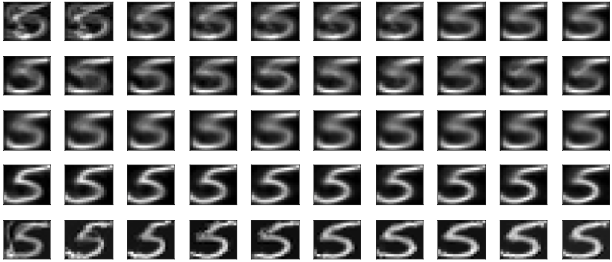
\includegraphics[width=3.5in]{pic_paper/small}\vspace{-.2cm}
\caption{(USPS Digits) Template estimation. From top to bottom: batch, online, \ISAEM,\ \SAEMVR\ and \FISAEM\ through 7 epochs. 
Batch method templates are replicated in-between epochs for a fair comparison with incremental ones. }\vspace{-.2cm}
\label{fig:results}
\end{center}
\end{figure}
As the iterations proceed, the templates become sharper.
Figure~\ref{fig:results} displays the virtue of the \SAEMVR\ and \FISAEM\ methods that obtain a more \textit{contrasted} and \textit{accurate} template estimate. 
The incremental and online versions are better in the very first epochs compared to the batch method, given the high computational cost of the latter. 
After a few epochs, the batch SAEM estimates similar template as the incremental and online methods due to their high variance. 
Our variance reduced and fast incremental variants are effective in the long run and sharpen the template estimates contrasting between the background and the regions of interest in the image.




\section{Conclusion}


This paper introduces a new class of two-timescale EM methods for learning latent variable models.
In particular, the models dealt with in this paper belong to the curved exponential family and are possibly nonconvex.
The nonconvexity of the optimization problem is tackled using a Robbins-Monro type of update, which represents the \textit{first level} of our class of methods.
The scalability with the number of samples is improved through a variance reduced and incremental update, the \textit{second} and last level of our newly introduced scheme.
The various algorithms are interpreted as scaled gradient methods, in the space of the sufficient statistics, and our convergence results are \emph{global}, in the sense of independence of the initial values, and \emph{non-asymptotic}, \ie true for any random termination number.
Numerical examples illustrate the benefits of our scheme on synthetic and real tasks.


%\section*{Acknowledgment}
%We thank Gersende Fort for the fruitful discussions on the methods.

\bibliographystyle{IEEEtran}
\bibliography{references}


\end{document}

